\documentclass[]{article}
\usepackage{amsmath}
\usepackage{graphicx}
\usepackage{caption}
\usepackage{mathtools}
\usepackage{cleveref}
\usepackage{courier}
\usepackage{subcaption}
\usepackage{units}
\usepackage{float}
\usepackage{placeins}
\usepackage{needspace}
\usepackage{amssymb}

\graphicspath{{/home/john/Documents/Python/Networks/figures/} }
%opening

\title{Network Project}
\author{John Norrie}

\begin{document}

\maketitle

\begin{abstract}
THIS IS MY ABSTRACT 
\end{abstract}

\section{Implementation of the BA Model}
The BA model is a randomly generated model, which usees a mdethod called preferential attachement to favour which nodes to connect to. This means that nodes with a high degree are more likely to be attached to be new nodes. The algorithm I used works as follows:
1. Set of an initial network a time $\mathcal{G_0}$.\\
\newline
2.Increment time t $\rightarrow$ t+1\\
\newline
3.Add one new vertex.
4. Add m edges as follows..
....\\...\\..\\
One of the biggest factors when creating this model is speed. The size of the networks we wish to analyse mean that a fast program is essential. The programme I developed creates a list of numbers, each couplet defining an edge. At the $k^{th}$ time step, a number is chosen at random (uniformly distributed) from this sequnce (x). then the number k and x are appended to the end of the list. This is carried out for $N$ time steps, after which the frequency of numbers are counted, and the outcome is the degree of each node. An example is shown below. \\
\begin{enumerate}
\item -$G=[0,1,0,2,1,2]$ is our starting graph, $N=3$, $m=3$
\item Add 2 new edges
\item 0 and 2 chossen randomly
\item $\Rightarrow G=[0,1,0,2,1,2,3,0,3,2]$
\item \text{Ending the iteration the counts are sorted, giving degree distribution:}\\ $deg(G)=[3,2,3,1]$
\end{enumerate}
This forces prereferntial attachement on the system, as if number $i<k$ appears more times in the sequence(e.i has more egdes attached), it is more likely to be chosen.
\subsection{Initial Graph}
There are a few points of ambiguity in this model. The first of which is with respect to $\mathcal{G}_0$. There is no explicit guidance on how to choose $\mathcal{G}_0\!$, however the choice of starting graph does have an affect. When deriving a solving the master equation for the system, we will use the approximation that $E(t)=mN(t) \!for\! large\! t$. However we can make this approximation exact by choosing an $\mathcal{G}_0$ such that $E(0)=mN(0)$.\\
In finding this, one assumption I would like to make is that ever node in $\mathcal{G_0}$ has the same degree. This make an easily programmably starting graph.This implies that $deg(n)=m\! for\! n \in \mathcal{G_0}$\\
There are many graphs with this property, however I would like to minimise the number of nodes in my starting graph(So our starting graph does not change our statistic) which implies we want a complete graph. THe algebra is as follow:
In a complete graph $E=\sum_{n=1}^{N} n-1 = \frac{N(N-1)}{2}$\\
\vspace{0.2cm}
And so $E(0)=mN(0) \Rightarrow \frac{N(0)(N(0)-1)}{2}=mN(0)$\\
\vspace{0.2cm}
$\Rightarrow N(0)^2 - (2m -1)N = 0$\\
\vspace{0.2cm}
$\Rightarrow N=0 (trivial) and N=2m+1$\\
\vspace{0.2cm}
Therefore choosing $\mathcal{G}_0$ to be a complete graph with $2m+1$ nodes is sufficient for the condition $E(0)=mN(0)$. Figure 1.1 shows the initial networks. 
\begin{figure}[htp]
	\centering
	%\includegraphics{figure_1.png}
	
	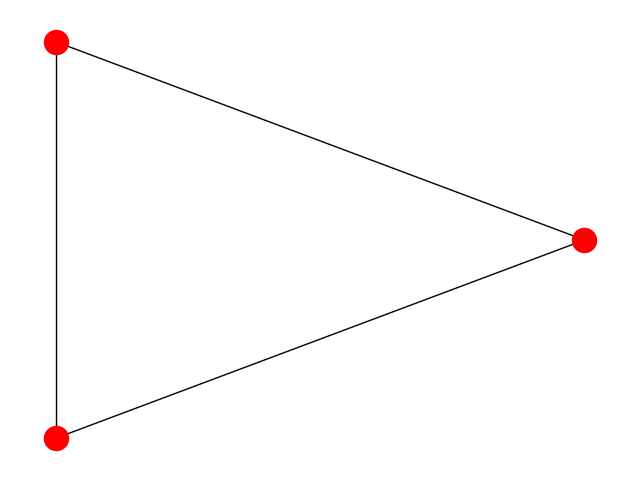
\includegraphics[width=.3\textwidth]{G0m=1.png}\hfill
	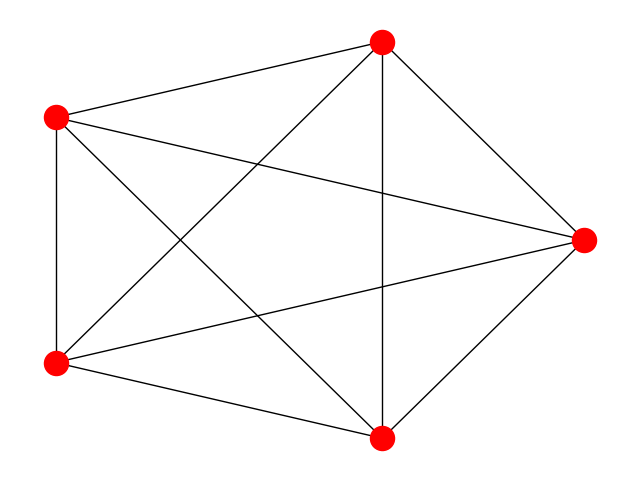
\includegraphics[width=.3\textwidth]{G0m=2.png}\hfill
	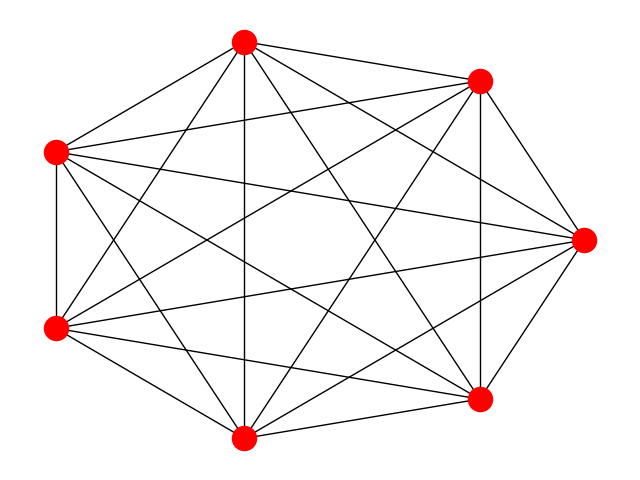
\includegraphics[width=.3\textwidth]{G0m=3.png}
	\caption{\textit{$\mathcal{G}_0$ for m=1,2,3 respectively.}}
\end{figure}
\subsection{Double Edges}
Another point of ambiguity is with regards to multiple egdes. In  the model, we have preferential attachement, which implies as we attach more edges to a node, it will be preferred even more when adding the node edge randomly. This "Rich get richer" attitude means that we are likely to get double edges when $m>1$. For instance, if a new node $k$ is added and attached to node $n<k$, then the probability of that happening again rises, implying we are more likely to see a double edge. This is especially true for small networks. Figure 1 shows a graph of 10 without addressing this issue and one where we do.
\begin{figure}[htp]
	\centering
	%\includegraphics{figure_1.png}
	
	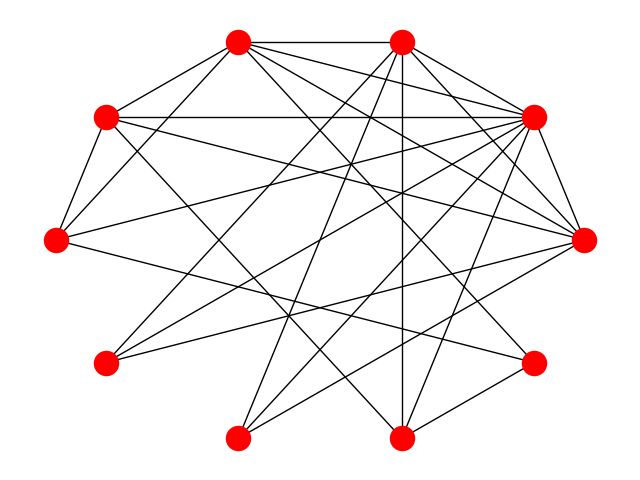
\includegraphics[width=.3\textwidth]{NonReplace.png}
	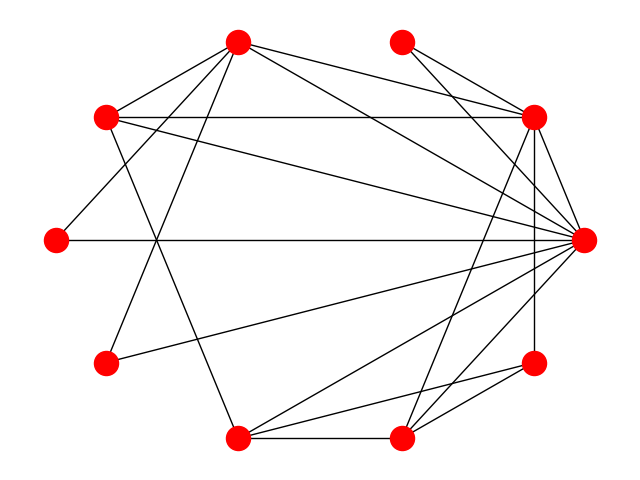
\includegraphics[width=.3\textwidth]{Replace.png}
	\caption{Left: \textit{Example graph of 10 nodes where we allows double edges(m=3). Not that there are nodes with degree less than m.}
		\\Right: \textit{Exampleof graph of 10 nodes. Note that all nodes have degree $>m$. Note that in both cases, I have not used $\mathcal{G}_0$, and instead have used a small initial graph to emphasise the difference in the cases.}}
\end{figure} 
This phenomena does not make sense in the circumstances for which this model is implemented, such as modeling the relationships between websites. Therefore I have decided to use the latter case. Also for large systems, theoretically there is no difference, since the probability of a node being chosen twice $\rightarrow 0$.
\subsection{Udpating Probabilities}

\subsection{Testing}
\subsection{Dynamic Testing}
\subsection{Macroscopic Testing}
\section{Theoretical Derivation of Degree}

There are a few ways of approximated the degree distribution $p(k)$, all three of which use the master equation: 
\begin{equation}
n(k,t+1)=n(k,t)+m\Pi(k-1,t)n(k-1,t)-m\Pi(k,t)n(k,t)+\delta_{k,m}
\end{equation}
Where $\Pi(k,t)$ is the probaility of an edge being attached to a node of degree $k$.
Since we are taking $\Pi(k,t) \propto k$, and that the probabilities are normalised, way get that:
\begin{equation}
\Pi(k,t)=\frac{k}{\sum_{k=1}^{\infty}{kn(k,t)}}
\end{equation}
Where $kn(k,t)$ is the number of degrees of the nodes of degree k. Also, each edge is reponsible for 2 degrees, and so:
\begin{equation}
\Pi(k,t)=\frac{k}{2E(t)}
\end{equation}
I have already discussed that $E(t)=mN(t)$ using the initial conditions chosen, and so $\Rightarrow \Pi(k,t)=\frac{k}{2mN(t)}$. Applying this to (1) the master equation becomes:
\begin{equation}
n(k,t+1)=n(k,t)+\frac{(k-1)n(k-1,t)}{2N(t)}-\frac{kn(k,t)}{2N(t)}+\delta_{k,m}
\end{equation}
Now we define the probability of choosing a degree randomly with degree $k$ at time $t$: 
\begin{equation}
p(k,t)=\frac{n(k,t)}{N(t)}\\
\end{equation}
So the master equation:
\begin{equation}
N(t+1)p(k,t+1)-N(t)p(k,t)=\frac{(k-1)}{2}p(k-1,t)-\frac{k}{2}p(k,t)+ \delta_k,m
\end{equation}
In order to go further, we assume that $p(k)$ has nice ergodic properties. This means that $p_{\infty}=lim_{t \rightarrow \infty} p(k,t)$\\, i.e. the limit converges. The Applying this to (6) the final form of our master equation becomes:
\begin{equation}
(N(t+1)-N(t))p_{\infty}(k)=-\frac{(k-1)}{2}p_{\infty}(k-1)-\frac{k}{2}p_{\infty}(k)+ \delta_k,m
\end{equation}
We note that $N(t)=t$  and so we find the final form of the master equation:
\begin{equation}
p_{\infty}(k)=\frac{1}{2}((k-1)p_{\infty}(k-1)-kp_{\infty}(k)) +\delta_{k,m}
\end{equation}
\subsection{Continuous Approximation}
Equation (7) can be used to find the degree distribution of the model.
An approximation of this distribution can be found using a limiting case, e.i. instead of have descrete degrees, we look at the continuous case $k+1 \rightarrow k + \Delta k$. (7) becomes:
\begin{equation}
{p(k) \approx \lim\limits_{\Delta k \rightarrow 0}\frac{-\frac{1}{2}((k-\Delta k )p_{\infty}(k-\Delta k)-kp_{\infty}(k)) +\delta_{k,m}}{\Delta k} }
\end{equation}
\begin{equation}
\Rightarrow p(k)\approx \frac{\partial kp_{\infty}(k)}{\partial k}
\end{equation}
By inspection (Looking for a solution of the type $k^{-\gamma}$), we find that $p(k) \propto k^{-3}$ is a solution.  This solution is very approximal. However once case we would expect to see such a distribution is for $m \rightarrow \infty$. As $m$ grows large, the difference between $k-1$ and $k$ grows small proportional to $k$, and so the limiting case becomes a reality.
\subsection{Difference Derivation}
It is poosible however to derive a solution from the difference equation. First we look at $k>m$ and rearrange (7):
\begin{equation}
\frac{p_{\infty}(k)}{p_{\infty}(k-1)}=-\frac{k-1}{2(k+1)}
\end{equation}
This may no look particularly helpful, however there is an identity of the Gamma function. The equation:
\begin{equation}
\frac{f(z)}{f(z-1)}=\frac{z+a}{z+b}
\end{equation}
Has the solution
\begin{equation}
f(z)=A\frac{\Gamma(z+1+a)}{\Gamma(z+1+b)}
\end{equation}
Therefore our difference equation has solution
\begin{equation}
p_{\infty}(k)=A\frac{\Gamma(k)}{\Gamma(k+2)}
\end{equation}
Using the identity $\Gamma(n)=(n-1)!$ for $n \in \mathbf{N}_0$, the solution becomes:
\begin{equation}
p_{\infty}(k)=\frac{A}{k(k+1)(k+2)}
\end{equation}
The constant $A$ can be found by looking at the boundary case, $k=m$, (7) becomes
\begin{equation}
p_{\infty}(m)=-\frac{m}{2}p_{\infty}(m)+1
\end{equation}
\begin{equation}
\Rightarrow p_{\infty}(m)=\frac{1}{m+2}
\end{equation}
This boundary conditon implies that 
\begin{equation}
A= 2m(m+1)
\end{equation}
Thus we derive the solution to the difference equation as:
\begin{equation}
p_{\infty}(k)=2m(m+1)/k(k+1)(k+2)
\end{equation}
I expect this distribution to be more accurate than that procured by the continuous approximation, as I have made less assumptions and approximations whilst deriving it.
\section{Comparison with Real Data}
Now I wish to compare these theoretical plots with the actual data captured by my model.\\
I shall run my programme for m=1,2,3 and for graphs of 10,000 nodes. I believe this is large enough to allow the ergodic properties of the probabilites, e.i. $p_{infty}(k)$ to arise.\\
 A key characteristic of the model is that as one increases the number of nodes in the graph ($N$), the maximum dregee $k_1$ observed also increase, which means no matter big the graph, the statistics towards the larger degrees will always be sparse. To combat this I ran the same experiment 100 times in order to build up a enough observatinos for large degree $k$, improving our statistic. Figure 3.1 shows the outcome. 
 
 \begin{figure}[H]
 	\makebox[\linewidth][c]{%
 		\begin{subfigure}{.6\textwidth}
 			\centering
		 	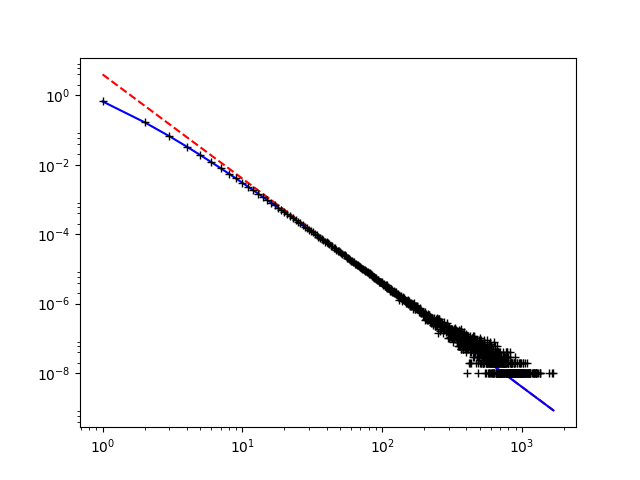
\includegraphics[width=\textwidth]{Datafit-m=1N=5.png}
 			\caption{$m=1$}
 		\end{subfigure}%
 		\begin{subfigure}{.6\textwidth}
 			\centering 
			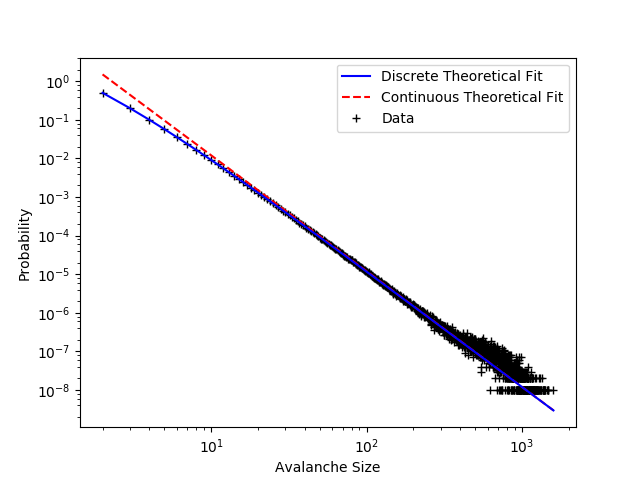
\includegraphics[width=\textwidth]{Datafit-m=2N=5.png}
 			\caption{$m=2$}
 		\end{subfigure}
 	}
 		\baselineskip
 	\makebox[\linewidth][c]{%
 		\begin{subfigure}{.6\textwidth}
 			\centering 
		 	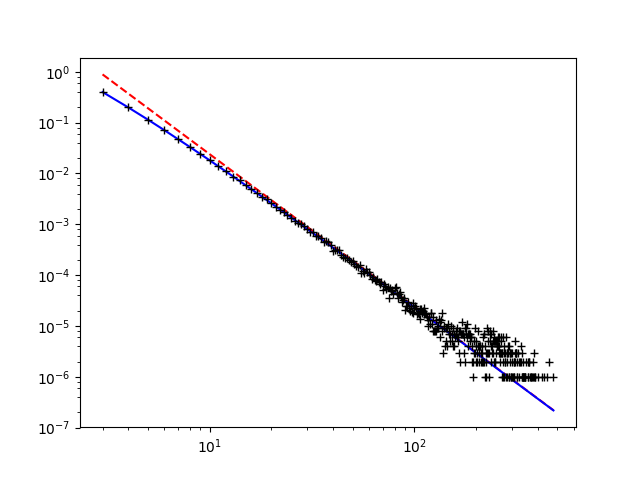
\includegraphics[width=\textwidth]{Datafit-m=3N=5.png}
 			\caption{$m=3$}
 		\end{subfigure}%
  		\begin{subfigure}{.6\textwidth}
  			\centering 
  			\includegraphics[width=\textwidth]{Datafit-m=4N=5.png}
  			\caption{$m=4$}
  		\end{subfigure}
 	}
 	\caption{The loglog plots of the raw data porbability distribuiton. This data was captured from networks of size $10^5$, and over $10^3$ traisl. a,b,c,d show the outcome for m=1,2,3,4 repectively.}
\end{figure}
 
Visually, one can see from that for small values of $k$, the probability fits our theoretical distribution perfectly. This is because there are a lot more nodes with degree small $k$, and so a lot more data is available, thus the distirbution is prominent. However, for large $k$ we have fewer and fewar nodes per degree, as predicted. This creates the 'fat tail' affect present on all three figures as seen in . \\
Notice as well that as m increase, our theoretical, and practical data moves closer to the line $p(k)=k^{-3}$. This verfifies the effect I would expect to see for large m.
\subsection{Statistical Approach}
I wish to analyse the model statistically. However, the 'fat tail' characteristic of the data means that the majority of our points lie near the origin. Therefore any statistical method I use will be dominated by the 'fat tail', and any conclusion I draw will be obscured. Log binning is way of mimising the 'fat tail, while keeping the necessary characteristics of the probability distribution.\\
When creating probability distributions from samples, data is put into bins, the frequency recorded and then normalised. In most cases we have a bin lengths constant, $b_{n+1}-b_{n}=:\Delta$. However in a log bin proccess, the bins have a relation $\frac{b_{n+1}}{b_n}=\Delta$. This means that the bins increase exponentially as the data grows larger. \\
This means for small $k$, where the data are plentiful, the bins are small to capture as much information as possible. However for large $k$,  where our data is sparse, the bins are large, meaning the a lot of data is grouped together to help gain insight into the behviour. The geometric mean of each bin is then plotted. Figure 4 shows how the log bin processes the raw data.
 \begin{figure}[H]
 	 	\makebox[\linewidth][c]{%
 	 		\begin{subfigure}{.6\textwidth}
 	 			\centering
 	 			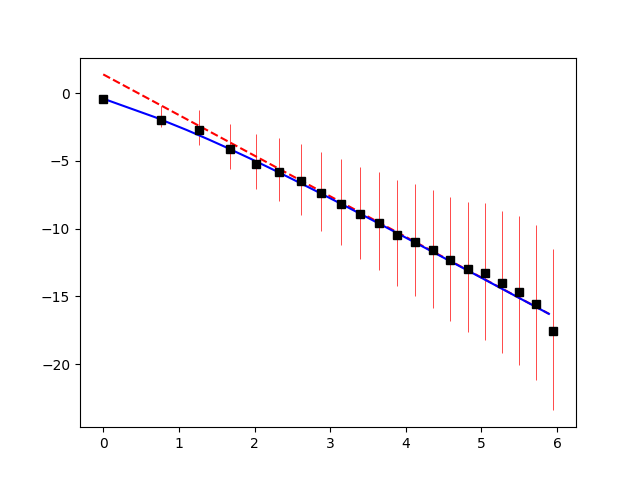
\includegraphics[width=\textwidth]{LogBin-m=1N=5.png}
 	 			\caption{$m=1$}
 	 		\end{subfigure}%
 	 		\begin{subfigure}{.6\textwidth}
 	 			\centering 
 	 			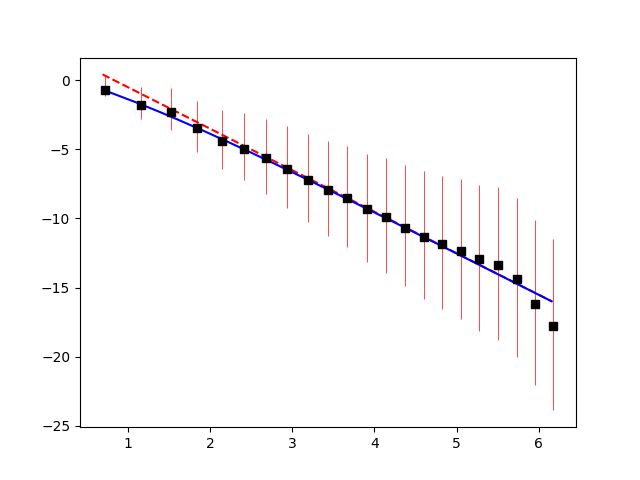
\includegraphics[width=\textwidth]{LogBin-m=2N=5.png}
 	 			\caption{$m=2$}
 	 		\end{subfigure}
 	 	}
  		\baselineskip
  		\makebox[\linewidth][c]{%
  			\begin{subfigure}{.6\textwidth}
  				\centering 
  				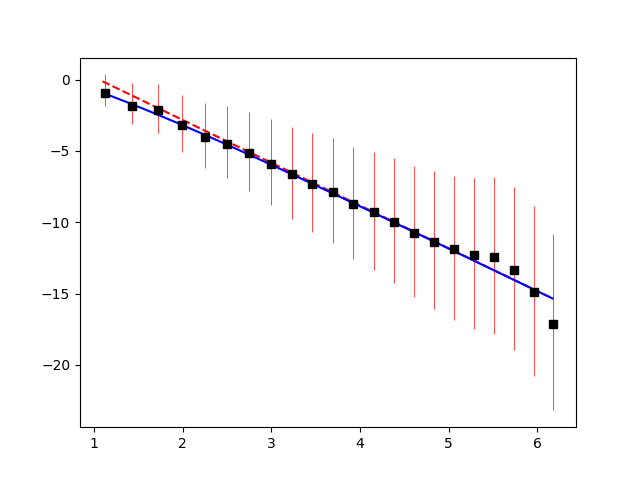
\includegraphics[width=\textwidth]{LogBin-m=3N=5.png}
  				\caption{$m=3$}
  			\end{subfigure}%
  			\begin{subfigure}{.6\textwidth}
  				\centering 
  				\includegraphics[width=\textwidth]{LogBin-m=4N=5.png}
  				\caption{$m=4$}
  			\end{subfigure}
  		}
  		\caption{Log binned probability distributions for $m=1,2,3,4$. The error bars show the logarithm of the deviation for a given data point. The increase of the bars implies that the variance of the data increases exponentially for large values of $k$}	 	
   \end{figure}
To statisitically analyse this data I plotted the theoretical fit and naive fit vs. the actual logbinned data. Assuming that my two fits and the actuall data are related, one would expect to see a linear regression between the variables. Figure 5 shows an example of this.
\begin{figure}[H]
	 	 	\makebox[\linewidth][c]{%

	 	 		\begin{subfigure}{.5\textwidth}
	 	 			\centering 
	 	 			\includegraphics[width=\textwidth]{LR-m=4LB.png}
	 	 		\end{subfigure}
	 	 	}
	 	   		\caption{The theoretical model(red) and the naive model(black) vs. the log binned, for $m=4$.
	 	   			}
\end{figure}
Fro firgure 5, one can see a definite linear relation in both cases. However to delve deeper, I calculated the least squares regression statistic($R^2$) for each of these relations. Using these I tested with the null hypothesis that there is no correlation(e.i. the slope between the two variable is 0) vs. the hypothesis that they are correlated using WHAT IS THE TEST CALLED????. All my statistics are listed below.
\begin{table}[H]
	\centering
	\caption{My caption}
	\label{my-label}
	\begin{tabular}{l|l|l|l|l|}
		\cline{2-5}
		& \multicolumn{4}{l|}{Linear Regression for Log Binned Data}            \\ \cline{2-5} 
		& \multicolumn{2}{l|}{Naive Fit} & \multicolumn{2}{l|}{Theoretical Fit} \\ \cline{2-5} 
		& $R^2$        & p-value         & $R^2$            & p-vaule           \\ \hline
		\multicolumn{1}{|l|}{m=1} & 0.992        & 2.71e-25        & 0.999            & 2.87e-40          \\ \hline
		\multicolumn{1}{|l|}{m=2} & 0.993        & 2.71e-25        & 0.999            & 2.86e-40          \\ \hline
		\multicolumn{1}{|l|}{m=3} & 0.993        & 2.72e-25        & 0.996            & 2.69e-28          \\ \hline
		\multicolumn{1}{|l|}{m-4} & 0.991        & 2.35e-24        & 0.994            & 2.72e-26          \\ \hline
	\end{tabular}
\end{table}
Examining these statisitcs, one can see that in all cases, the p-statistic is very small. Infact we can reject the null hypothesis with a confidence level of 1.e-25 for all stastics. This impies that there is definitly correlation, and therefore both models would suffice.\\
To analyse which model is better one needs to examine the $R^2$ terms. For all $m$, the $R^2$ statistic is great for the theoretical fit, than that of the naive fit. This implies that the theoretical fit is better.
Note that the difference $R^2$ statistics for the two fits shrinks. This is more evidence that points towards the phenomena that as m increases our two fits converge.    
\section{Finite Size Effect}
\subsection{Theoretical Derivation}
I wish to find how the greatest degree $k_1$. To do this I look at the master equation in the form:
\begin{equation}
N(t+1)p(k,t+1)-N(t)p(k,t)=-\frac{(k-1)}{2}p(k-1,t)-\frac{k}{2}p(k,t)+ \delta_{k,m}	
\end{equation}
Again taking the limiting case, but this time in both $k$ and $t$:
\begin{equation}
N(t+\Delta t)p(k,t+\Delta t)-N(t)p(k,t)=-\frac{1}{2}((k-\Delta k)p(k-\Delta k,t)-kp(k,t))+ \delta_{k,m}		
\end{equation}
To go further I make some assumptions. First of all we wish to express equation in terms of partial derivatives. And so we assume that $\Delta k ~ O(\Delta t^{\alpha})$, e.i. when $\Delta t \rightarrow 0 \Rightarrow \Delta k \rightarrow 0$. \\
Another assumption is that we can ignore the  $\delta_{k,m}$ term. Doing this means we can take the derivative limit:
\begin{equation}
	\frac{N(t+\Delta t)p(k,t+\Delta t)-N(t)p(k,t)}{\Delta t}=-\frac{(k-\Delta k)p(k-\Delta k,t)-p(k,t)}{2 \Delta k}
\end{equation}
Taking the limit:
\begin{equation}
\frac{\partial (N(t)p(k,t))}{\partial t}= -\frac{1}{2}\frac{\partial(kp(k,t))}{\partial k}
\end{equation}
Solving this equation we first use the fact that $N(t)=t$, and  the ansatz that $p(k,t)=f(t)k^{-\gamma}$.
\begin{equation} 
k^{-\gamma}\frac{\partial (tf(t))}{\partial t}= -\frac{f(t)}{2}\frac{\partial k^{1-\gamma}}{\partial k}
\end{equation}
\begin{equation}
	\Rightarrow \frac{\partial (tf(t))}{\partial t}= -\frac{(1-\gamma)f(t)}{2}
\end{equation}
By inpspection a solution to this equation is $f(t) \propto t^{-\alpha}$:
\begin{equation}
\Rightarrow  \frac{\partial (t^{1-\alpha})}{\partial t}= -\frac{(1-\gamma)t^{-\alpha}}{2}
\end{equation}
\begin{equation}
\Rightarrow 1- \alpha= -\frac{(1-\gamma)}{2}
\end{equation}
Rearranging we obtain $\gamma$ in terms of $\alpha$
\begin{equation}
\gamma = 3 - 2\alpha
\end{equation}
And so we find the behaviour of the probability solution approximates to:
\begin{equation}
p(k,t) \propto (\frac{k^2}{t})^{\alpha}k^{-3} 
\end{equation}
We know that for large $t$, $p(k,t) \approx k^-3$ we can assume that
\begin{equation}
 \frac{k^2}{t} \propto 1 \Rightarrow k \propto \sqrt{t}
\end{equation}
Therefore we expect the largest degree $k_1$ to scale with the square root of $N(t)$. One might be tempted to try and derive $\alpha$, and therefore have an exact theoretical model of how the the degree distribution is affect by the finite size. However in practice this is particularly hard, and many of the features of the degree distribution have already been explained. Therefore I shall not be deriving this in this report.
\subsection{Experimental Data}
To test how $k_1$ scales $N$, I ran my program for $N=10^2, 10^3, 10^4, 10^5$, collecting the maximum degrees. I focus on $m=$, the maximum $m$ I recorded because due the the fact that there are more edges, we expect more larger degree observations, giving us a clearler idea of how degree distribuiton behaves in the fat tail. This can be seen in figure 1. The tail for $m=4$ is more defined than that of $m=1,2,3$. We are interested in these larger degrees, as they obviously depend a lot more on the finite size of the graph. The fact that this is an extreme statistic means that it is very intermittent, and therefore one would expect to see a lot of variance between trials. Therefore I repeated this experiment 100 times, and took the median to help gain a more appropriate statistics. Figure 4 shows the result. 
\begin{figure}[H]
	\centering
	%\includegraphics{figure_1.png}
	
	\includegraphics[width=.5\textwidth]{k1.png}
	\caption{The median for $N=1,2,3,4$ and a naive fit of $k1 \propto \sqrt{N}$ are plotted. The error bars represent $\sqrt{deviation}$ from our most extreme statistics and the  median.}
\end{figure}
Figure 4 shows that the real data is in accordance with our theoretical model. With respect to the error bars, one can see that the length above each point($\sqrt{max(k_1(N))-<k_1(N)>}$) is vastly greater than that of the below errorbar. This implies that our statistics have much variance above the, than below. This is why I used the median instead of the mean, as the mean would be skewed by this fact.\\
As the error bars show there is a lot of uncertainty in this relationship, primarily due to the fact e are measuring an extreme statistic for which the occurence is very rare and sporadic. The best way to overcome this is to use more trails.
\subsection{Data Collapse}
Since we now know how the degree distribution depends on $k$, $m$ and $N$, I can perform a data collapse. I concentrate on m=4, as it gives me better statistical data for large degree sizes. I vary $N=10^2, 10^3, 10^4, 10^5$. Figure 5 shows a plot of how the uncollapsed degree distributions correlate. 
\begin{figure}[H]
	\centering
	%\includegraphics{figure_1.png}
	
	\includegraphics[width=.7\textwidth]{Collapse11.png}
	\caption{The median for $N=1,2,3,4$ and a naive fit of $k1 \propto \sqrt{N}$ are plotted. The error bars represent $\sqrt{deviation}$ from our most extreme statistics and the  median.}
\end{figure} 
First I collapse the probability distribution in k by dividing through by my theoretical prediction:
\begin{equation}
	c_k(N)=\frac{p_{data}(k)}{p_{theory}(k)}
\end{equation}
Figure 5 shows the outcome of this proccedure.
\begin{figure}[H]
	\centering
	%\includegraphics{figure_1.png}
	
	\includegraphics[width=.7\textwidth]{Collapse2.png}
	\caption{The median for $N=1,2,3,4$ and a naive fit of $k1 \propto \sqrt{N}$ are plotted. The error bars represent $\sqrt{deviation}$ from our most extreme statistics and the  median.}
\end{figure}
Now I collapse in N. To do this I use the relation I earlier derived of how the $k_1$ scales with $N$. I stretched the degrees observed by a factor of $N^{-\frac{1}{2}}$. Figure 7 shows the full collapse.
\begin{figure}[H]
	\centering
	%\includegraphics{figure_1.png}
	
	\includegraphics[width=.7\textwidth]{Collapse1.png}
	\caption{The median for $N=1,2,3,4$ and a naive fit of $k1 \propto \sqrt{N}$ are plotted. The error bars represent $\sqrt{deviation}$ from our most extreme statistics and the  median.}
\end{figure}
\section{Random Attachement}

\end{document}
